\documentclass[11pt]{article}
% RFP specifically says to use 11 point type and 1 inch margins
\usepackage{graphicx}
\usepackage{epsf,color}
\textwidth=6.5in\oddsidemargin=0in \evensidemargin=0in \topmargin
0pt \advance \topmargin by -\headheight \advance \topmargin by
-\headsep \textheight 9.0in

%\textwidth=6.5in\oddsidemargin=0in \evensidemargin=0in \topmargin
%0pt \advance \topmargin by -\headheight \advance \topmargin by
%-\headsep \textheight 8.9in

\usepackage{amsmath}
\usepackage{graphicx}
\usepackage{dcolumn}
\usepackage{multirow}
\usepackage{wrapfig}
\usepackage[compact]{titlesec}

%\usepackage[plain]{fullpage}
\usepackage{amsfonts}
%\usepackage{lastpage}
%\usepackage{fancyhdr}

\usepackage[version=3]{mhchem} 
% you can use this command to skip chunks of your document
% just put the command around the chunk like this
% \comment{ ...the chunk... }
\newcommand{\comment}[1]{}

%\newcommand{\MarginPar}[1]{\hspace{1sp}\marginpar{\tiny\sffamily\raggedright\hspace{1sp}#1}}
\setlength{\marginparwidth}{0.75in}
\newcommand{\MarginPar}[1]{\marginpar{%
\vskip-\baselineskip %raise the marginpar a bit
\raggedright\tiny\sffamily
\hrule\smallskip{\color{red}#1}\par\smallskip\hrule}}

\definecolor{drkgrn}{rgb}{0.043,0.341,0.2274}
\newcommand{\remrg}[1]{ {\it \color{drkgrn} \{#1 -RG\}}}

%\renewcommand{\baselinestretch}{1.05} % = 1.0 Single space; = 2.0 Double
\renewcommand{\baselinestretch}{1.0} % = 1.0 Single space; = 2.0 Double

%\renewcommand{\refname}{Literature Cited}
%------------------------

%\pagestyle{empty}  % No page numbers
%\textfloatsep 0mm
%\abovecaptionskip 1mm

\begin{document}

%\pagestyle{plain}
%\pagenumbering{roman}
\begin{center}
{\Large{\textbf{Point defect formation kinetics}}}
\end{center}

 
\subsection*{Point defect formation in thin-film photovoltaics:}

Another application where there is a complex parameter estimation
problem is the formation of point defects in thin-film photovoltaic
materials. 

Thin film photovoltaic (PV) devices have attracted research attention
as a way to dramatically reduced the cost of solar panels. These
materials compete with traditional crystalline silicone based on
efficiency but use far less ($\mathcal{O}(1\%)$, \cite{find})
material. Leading thin film technologies include absorbers based on
cadmium telluride (CdTe), CIGS, and CZTS \cite{JiangY13}. In contrast
to the exotic elements in CdTe and CIGS, CZTS ($Cu_2ZnSnS_4$) is
comprised of relatively abundant and benign constituents. However,
despite considerable attention CZTS development is still not mature
relative to CdTe technology. The performance is sensitive to the
fabrication process: leading demonstrations for CZTS successful
fabrication processes include depositing the film on a substrate via
solution-processing (11\% conversion efficiency) \cite{Todorov13},
co-evaporation (9.15\% efficiency \cite{Repins12})) and vacuum
process (8.4\% efficiency, \cite{Shin11}). Despite theoretical
efficiencies exceeding 30\%, developing optimum processing conditions
that realize the potential remain elusive. For our present
  purpose, the challenge is {\bf given a set of measurements of bulk
    properties that result from uncertain and time-varying process
    conditions, can we refine estimates of the model parameters
    sufficiently to be able to predict the time-varying process
    conditions most likely to result in a desirable configuration}. 

  Unlike crystalline silicone that is explicitly doped with
  phosphorous or boron to create n-type or p-type semiconductors, CZTS
  is `self-doped' through point defects in the kesterite
  crystal. Creation of these defects (vacancies, antisite and
  interstitial) , particularly the $Cu_{Zn}$ antisite defect for
  p-type doping in CZTS, results in an increase in carrier
  concentration and semiconductor behavior \cite{JiangY13}.  However,
  other defects have been identified as reducing carrier lifetime
  through providing recombination centers. Further, a system such as
  CZTS has a complicated phase diagram with a narrow region where the
  CZTS phase is present. The effects of the secondary phase presence
  on device performance is throughly described in, e.g.,
  \cite{Flammersberger}, but are largely detrimental to device
  performance. Grain boundaries between phases also alter the driving
  force for point defect migration. \cite{Kolluri12} looked into
  transport of delocalized defects at interfacial grain boundaries for
  CuNb and found that it can be modelled as a complication on
  localized defect migration and successfully treated based on
  transition state theory with temperature dependent
  prefactor. Whether in the pure crystal or at a phase boundary, point
  defects in close proximity can interact, e.g., a vacancy and
  interstitial defect can combine to heal the crystal. 

  From an analysis perspective, assembling a comprehensive model
  requires treatment multiple physical processes with poorly
  understood parameters. In the remainder of this section, we will
  provide an overview of the building blocks of such a model. Two
  approaches are available: detailed electronic structure calculations
  \footnote{Walsh, A., Chen, S., Wei, S.-H. and Gong, X.-G. (2012),
    Kesterite Thin-Film Solar Cells: Advances in Materials Modelling
    of Cu2ZnSnS4. Adv. Energy Mater., 2: 400–409. doi:
    10.1002/aenm.201100630} provide a wealth of information indicating
  the important physical processes and configuration effects, but are
  unable to connect back to processing through long term dynamics. An
  alternate approach is to utilize continuum descriptions of
  point-defect formation and interaction; however, many of the
  parameters in such a description are difficult to identify,
  underscoring our interest in this approach.

\begin{itemize}
  \item Firstly, the surface process by which metal flux from the vapor
  stream are added to the crystal. This is process dependent, although
  well established models are available. \marginpar{at least CVD is,
    although co-evaporation is more common}

\item Secondly, the formation and interactions of the point defects
  within the film can be expressed in terms of continuum point defect
  concentration/number densities. Static electronic structure
  calculations can estimate the enthalpy difference when a given point
  defect is formed, but these calculation are of little practical use
  to compute the dynamics of the system. Instead, `pseudo-reactions'
  based on Arrhenius form are written. For example, a simple model of a
  MS system (a realistic description of the full CZTS system includes
  many more relations) can be described by a simplistic system of four
  reactions expressing an oxidation reaction, the Schottky disorder
  and creation of anion vacancies:

\begin{eqnarray*}
\ce{ \tfrac{1}{2} S2 -> S_s^x + V_m^{''} + 2 h^+ } \\
\ce{ NULL -> V_m^{''}+ V_s^{$\cdot \cdot$} } \\
\ce{ NULL -> e^' + h^{$\cdot$} } \\
\ce{ S_s^x -> \tfrac{1}{2} S2 + V_s^{$\cdot \cdot$} + 2 e^- }.
\end{eqnarray*}

Where the rate of the $\alpha^{\mathrm{th}}$ reaction is approximated
by the Arrhenius form and the law of mass-action based on defect
number densities:
\begin{equation}
  \label{eq:1}
  k_\alpha e^{-(E_a)_\alpha/(RT)}.
\end{equation}

Solution of this system yields the $e$ and $h$ carrier
concentrations that are used to assess device performance based on the
partial pressures resulting from the metal fluxes. However, the
activation energy and pre-exponential factor are difficult to
estimate. Using the enthalpy difference across the reaction --- that
can be estimated from electronic structure calculations, although the
energy barrier is not so easily attainable --- provides
the correct equilibrium solution, but tells us little about the
dynamics. Thus we have only the coarsest estimate of the parameters
available as priors.

\item The reactions above involve gas-phase species concentrations that must
be determined from the metal flux at the film surface. Diffusion of
these gasses into the film can be treated with a gradient-based
(Fickian) approximation. 

\item Transport of the point defects within the crystal occurs by in two
regimes. Solid state diffusion is frequently approximated using a
Fickian treatment, however for point defects this is insufficient to
account for their migration along grain boundaries, where, as
suggested earlier, the transport mechanism changes and becomes
delocalized. Higher probability of the defect moving along the grain
boundary can be captured by a stochastic model more naturally than a
deterministic treatment. 

\item The importance of grain boundaries for transport requires a model for
grain nucleation and growth that is notoriously difficult to capture
deterministically; stochastic models have been much more successful \cite{Koptelov84}.
\marginpar{L. Petzold  has literature on how to connect such components}

\end{itemize}

Collecting these physics, a reasonable stochastic PDE governing the
number density of a point defect, $\phi$ as a function of space-time
within the film can be written as:
\begin{equation}
  \label{eq:3}
  \phi_t = S^\phi - D \phi_{xx}  + T^\phi,
\end{equation}
where $s^\phi$ is the net rate of formation/destruction of the defect
due to the system of reactions describing the point defect chemistry
and interaction, the second term on the rhs is a deterministic
transport contribution, and the final term on the rhs represents
stochastic transport that is active only in the vicinity of a grain
boundary. 

Auxiliary simulations are necessary to provide the boundary
conditions; e.g., \cite{cigs-parallel-simulation} and a model for
grain growth. The latter, following seeding from stochastic processes
dependent on the local elemental composition can be treated with a
moving front method. 

This problem has several aspects that differentiate it from the other
applications that we would like to highlight: 
\begin{itemize}
\item It is has an inherently stochastic nature
\item It exhibits very large uncertainty in relatively few parameters
\item It is somewhat less well studied than the combustion system,
  leading to a significant opportunity for model insufficiency ---
  providing an opportunity to test the robustness of mechanisms to
  detect when model is inconsistent with data)
\end{itemize}

\remrg{Workflow: cf. experiments to pin down uncertainty in kinetic
parameters, transport probabilities, etc. Then search for processing
pathway that provides optimum result given remaining uncertainty in
parameters. Can we use similar sampling ideas for the final
  optimization step?}

\emph{Measurements: carrier concentration; resistance; conductivity;
  changes\ldots}


%
%{\it First principles calculations have suggested that there is a
%  theoretical configuration for such materials as CZTS and CIGS that
%  leads to a combination of carrier concentrations, mobility and
%  minority carrier lifetime that would provide exceptional device
%  performance. However, the question of how to control process
%  conditions during film deposition to arrive at such a configuration
%  remains open. Modelling the kinetics of point defect formation
%  through pseudo-reactions results in a system of differential
%  equations that are tightly coupled and indicate the resulting
%  properties have a non-trivial relationship to the intrinsic
%  defects.  Electronic structure calculations can provide an estimate
%  fo the energy difference when defects are formed but the kinetic
%  parameters (energy barriers) are the result of indirect measurements.}


Direct measurement of the concentration of arbitrary point defects is
difficult and must be inferred from more easily observed
characteristics, leading a model for the observation process $h(x)$
that may be quite complicated and the result of a non-trivial
simulation.  For example, majority carrier concentration, electron or
hole mobility, capacitance can be measured, but these are all
indicators of the final point defect configuration that results from
the process rather than measures of the individual formation
rates. With significantly more effort, the dependence of the film
conductivity on temperature provides an indirect measure of the
activation energy for carrier concentration: this is related to the
kinetic parmeters of the governing defect concentration(s).  A variety
of simulation/experiment pairs are desirable to increase sensitivity
to the various parameters separately:

%\begin{figure}[h]
%  \centering
%  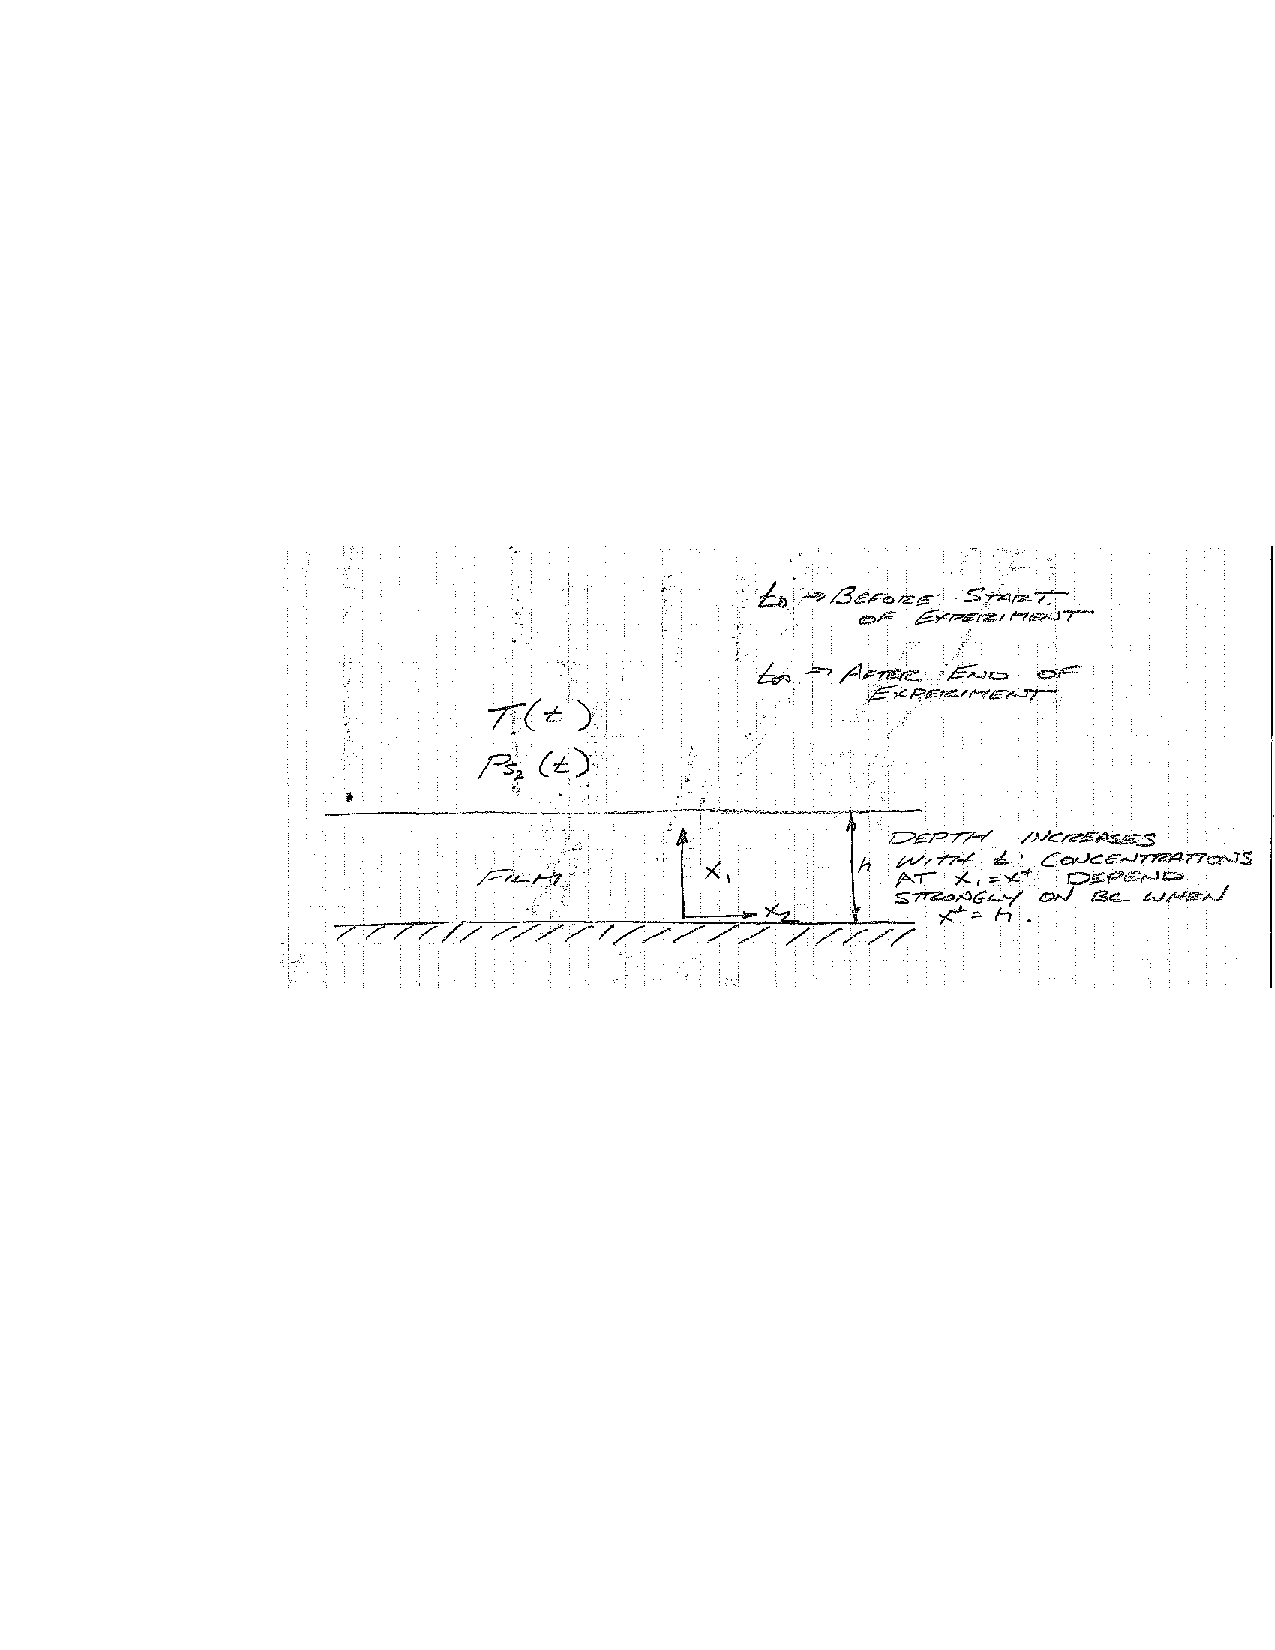
\includegraphics[width=0.8\textwidth]{pd_sketch.pdf}
%  \caption{Sketch of film deposition}
%  \label{fig:film}
%\end{figure}


\remrg{The experimental process parameters could be
  thought of as either an uncertain input, albeit not one we're
  trying to constrain, or as an observable. At first glance the latter
  seems more appropriate.}

%\begin{table}[h]
%  \centering
%  \begin{tabular}{l l l l l}
%    Level in hierarchy & Model inputs & Observables & Processes
%    addressed \\
%    \hline
%    0-D, steady & $(E_a)_\alpha$  & $p_{S_2}(t_0)$ & Equilibrium
%    concentrations \\
%    & & $T(t_0)$ & \\
%    & & $h^+(t_\infty)$ & \\
%    & & $e^-(t_\infty)$ & \\
%    \hline
%    0-D, unsteady & $(E_a)_\alpha$& $p_{S_2}(t)$ & Time dependent
%    bcs \\
%    & $k_\alpha$ & $T(t)$ & Quasi-equilibrium states \\
%    & & $h^+(t_\infty)$ & Dependence on ICs \\
%    & & $e^-(t_\infty)$ & \\
%
%    \hline
%    1-D, unsteady & $(E_a)_\alpha$& $p_{S_2}(t)$ & Time dependent
%    bcs \\
%    & $k_\alpha$ & $T(t)$ & Quasi-equilibrium states \\
%     & $D_j$ &$h^+(t_\infty)$ &  Dependence on ICs \\
%     & & $e^-(t_\infty)$ & Finite rate transport \\
%     & && Time dependent bcs coupled \\
%     & & &    to finite rate transport \\
%  \end{tabular}
%  \caption{Inputs, observables and physical processes included in
%    possible PD simulation hierarchy. }
%  \label{tab:pdh}
%\end{table}


\bibliographystyle{plain}

\bibliography{pd} 



\end{document}
